%%%%%%%%%%%%%%%%%%%%%%%%%%%%%%%
%This is the article LaTeX template for RSC journals
%Copyright The Royal Society of Chemistry 2010
%%%%%%%%%%%%%%%%%%%%%%%%%%%%%%%


\documentclass[8.5pt,twoside,twocolumn]{article}
\oddsidemargin -1.2cm
\evensidemargin -1.2cm
\textwidth 18cm
\headheight 1.0in
\topmargin -3.5cm
\textheight 22cm
\usepackage[super,sort&compress,comma]{natbib} 
\usepackage{graphicx}
\usepackage{color}
\usepackage{mhchem}
\usepackage{times,mathptmx}
\usepackage{sectsty}
\usepackage{balance} 

\usepackage{graphicx} %eps figures can be used instead
\usepackage{lastpage}
\usepackage[format=plain,justification=raggedright,singlelinecheck=false,font=small,labelfont=bf,labelsep=space]{caption} 
\usepackage{fancyhdr}
\pagestyle{fancy}

\begin{document}

\thispagestyle{plain}
\fancypagestyle{plain}{
\fancyhead[L]{\textit{\small{\textbf{Redes Neuronales}}}}
\fancyhead[C]{\textbf{Trabajo Pr\'actico I }}
\fancyhead[R]{\textbf{Jennifer Maldonado}}\vspace{0.5cm}}
\renewcommand{\thefootnote}{\fnsymbol{footnote}}
\renewcommand\footnoterule{\vspace*{1pt}% 
\hrule width 3.4in height 0.2pt \vspace*{2pt}} 
\setcounter{secnumdepth}{5}



\makeatletter 
\def\subsubsection{\@startsection{subsubsection}{3}{10pt}{-1.25ex plus -1ex minus -.1ex}{0ex plus 0ex}{\normalsize\bf}} 
\def\paragraph{\@startsection{paragraph}{4}{10pt}{-1.25ex plus -1ex minus -.1ex}{0ex plus 0ex}{\normalsize\textit}} 
\renewcommand\@biblabel[1]{#1}            
\renewcommand\@makefntext[1]% 
{\noindent\makebox[0pt][r]{\@thefnmark\,}#1}
\makeatother 
\renewcommand{\figurename}{\small{Fig.}~}
\sectionfont{\large}
\subsectionfont{\normalsize} 

\fancyfoot{}
\fancyfoot[RO]{\footnotesize{\sffamily{1--\pageref{LastPage} ~\textbar  \hspace{2pt}\thepage}}}
\fancyfoot[LE]{\footnotesize{\sffamily{\thepage~\textbar\hspace{2.45cm} 1--\pageref{LastPage}}}}
\fancyhead{}
\renewcommand{\headrulewidth}{1pt} 
\renewcommand{\footrulewidth}{1pt}
\setlength{\arrayrulewidth}{1pt}
\setlength{\columnsep}{6.5mm}
\setlength\bibsep{1pt}

\twocolumn[
  \begin{@twocolumnfalse}
  \vspace{0.2cm}
  \noindent \normalsize{
        La hoja de c\'alculo denominada "clima\_numerico" contiene los mismos patrones
representados por sus valores num\'ericos originales (en el caso de los atributos
humedad y temperatura) o por valores enteros asociados a la categor\'ia
correspondiente (0=falso y 1= verdadero; 0=lluvioso, 0.5=nublado; 1=soleado).
Utilice los patrones de la hoja "clima\_numerico" para entrenar un perceptr\'on que
permita predecir, a partir de una condici\'on clim\'atica dada, si se jugar\'a al golf o no
  }
  \vspace{0.5cm}
  \end{@twocolumnfalse}
  ]


\section{Analice si se producen variantes con respecto a los par\'ametros del algoritmo de entrenamiento.}
      
        Se realiz\'o la ejecucion de 50 iteraciones por cada alfa, modificando la cantidad m\'axima de iteraciones
        de forma incremental, el ejercicio por tener pocos n\'umero de filas (patrones) convergi\'o a la soluci\'on
 sin llegar al m\'aximo n\'umero de iteraciones s\'olo para los alfa -0.5, 0.3, 0.4, 0.5. Es importante mencionar que 
los datos no se encontraban normalizados, el promedio de los resultados puede visualizarse en la Tabla 1 y los 
datos se pueden obtener en el siguiente enlace: http://bit.ly/15xcRzx. La figura 1 muestra la relaci\'on entre el valor
alfa y el n\'umero de iteraciones que le toma llegar a la soluci\'on que permita discriminar.

 	\begin{figure}[h]
	  \centering
	  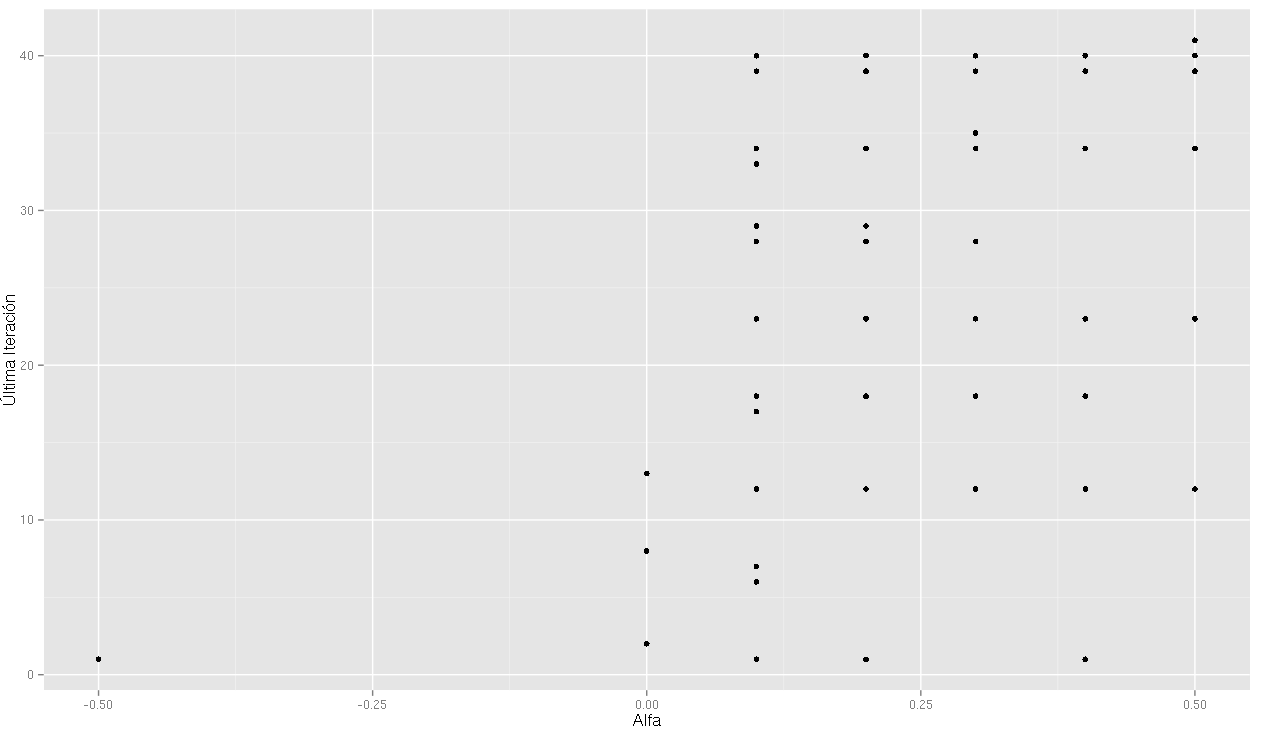
\includegraphics[scale=0.2]{clima_alfa_iteracion1a.png}
	  \caption{Comparaci\'on entre el valor del par\'ametro Alfa y el n\'umero de Iteraciones que realiza para llegar a la soluci\'on}
	  \label{fgr:alfaIteracion}
	\end{figure}

        \begin{table}[h]
        \small
        \caption{ Alfas, Promedio de Iteraciones, Cantidad de Aciertos (promedios) }
        \label{tbl:example}
        \begin{tabular*}{0.5\textwidth}{@{\extracolsep{\fill}}llll}
        \hline
        Aciertos (Promedio) & alfa & Ite $<$ Max\_It & Ite (Promedio)\\
        \hline
        2 & 0.2 & $50/50$ & 25.5 \\
        2 & 0.3 & $50/50$ & 24.2 \\
        2 & 0.1 & $50/50$ & 23.64 \\
        2 & 0.5 & $50/50$ & 22.06 \\
        2 & 0.4 & $50/50$ & 19.04  \\
        2 & -0.5 & $1/50$ & 1 \\
        1.54 & -0.1 & $0/50$ & 2550 \\
        1.6 & -0.2 & $0/50$ & 2550 \\
        1.46 & -0.3 & $0/50$ & 2550 \\
        1.42 & -0.4 & $0/50$ & 2550 \\
        \hline
        \end{tabular*}
        \end{table}

La figura 2  muestra un promedio de 50 iteraciones por cada valor de alfa, se muestra el sub conjunto donde el perceptron
converge a la soluci\'on y el n\'umero de iteraciones es menor que el valor m\'aximo estipulado como par\'ametro inicial.
Para valores cercanos a 0 de alfa tienen un menor n\'umero de iteraci\'on, donde el valor m\'inimo es 7.66 y su m\'aximo valor
25.5 para valores de alfa sobre 0.3 a 0.4. 

	\begin{figure}[h]
	  \centering
	  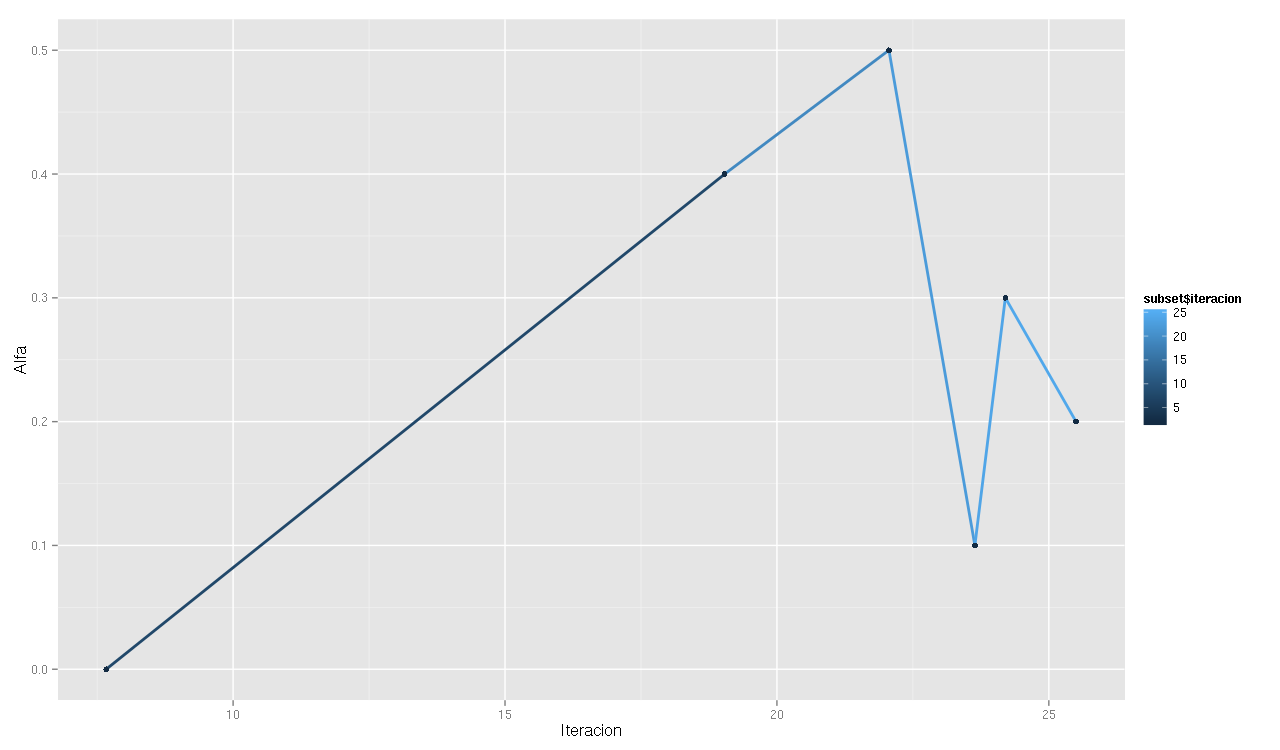
\includegraphics[scale=0.2]{adult_alfa_iteracion_itefinal.png}
	  \caption{Comparaci\'on entre el valor del par\'ametro Alfa y el n\'umero de Iteraciones que realiza para llegar a la soluci\'on}
	  \label{fgr:alfaIteracion}
	\end{figure}

        En todas las variaciones de alfa desde 0.1 a 0.5 el perceptron obtiene la soluci\'on antes de llegar a la m\'axima iteraci\'on. 
        La tercera columna muestra el n\'umero de iteraciones que realiz\'o sin llegar a la m\'axima iteraci\'on.
        La \'ultima columna muestra la iteraci\'on promedio por lo que se puede afirmar que sin escalar los datos, el algoritmo realizar\'a
aproximadamente desde 19 hasta 26 iteraciones. A diferencia de utilizar los datos escalados,  se observa que se reducen dr\'asticamente el n\'umero 
de iteraciones promedio pasando a tener un m\'inimo de 3 hasta 11 iteraciones. Esto se puede observar mejor en la siguiente secci\'on. 

       
 \section{Analice si es necesario escalar los datos de entrada.}
    Luego de haber escalado los datos a un intervalo $[0,1]$ comparando los resultados anteriores.  se puede observar que:
    \\ Se reduce el n\'umero de iteraciones un 50\% si los datos estan escalados, por lo tanto el tiempo de c\'omputo es menor. 
    \\ El n\'umero de Aciertos se ve afectado, reduciendo un poco la cantidad de aciertos para todos los alfas. 
sin embargo el n\'umero de patrones es peque\~no para afirmar alguna premisa sobre este punto.

        \begin{table}[h]
        \small
        \caption{ Alfas, Promedio de Iteraciones, Cantidad de Aciertos (promedios) }
        \label{tbl:example}
        \begin{tabular*}{0.5\textwidth}{@{\extracolsep{\fill}}llll}
        \hline
        Aciertos (Promedio) & alfa & Ite $<$ Max\_It & Ite (Promedio)\\
        \hline
        1.1  & 0.5 & $50/50$ & 11.96 \\
        1.0476  & 0.4& $21/50$ & 8.4285  \\
        1.4615 & 0.3 & $13/50$ & 2.8461 \\
        1.5384 & 0.1 & $13/50$ & 3.8461 \\
        0.8333 & 0.2 & $12/50$ & 3.25 \\
        1 & -0.4 & $1/50$ & 1 \\
        1.5 & -0.1 & $4/50$ & 1.5 \\
        1.46 & -0.3 & $3/50$ & 1.333 \\
        1.02 & -0.2 & $1/50$ & 1 \\
        1 & -0.5 & $0/50$ & 2550 \\
        \hline
        \end{tabular*}
        \end{table}

    \section{Es posible clasificar todos los patrones correctamente ingresando todos los de una clase primero y luego todos los de otra clase?}

    No, adem\'as el perceptron utiliza un tiempo mayor al promedio.\%

    En la tabla 3 se puede observar como var\'ia con respecto a los diferentes par\'ametros, adem\'as visualizamos que alfa es
m\'as conveniente utilizar para obtener una buena relaci\'on entre la mayor cantidad de aciertos y el menor n\'umero de iteraciones. 
\\
En todas las iteraciones se detiene antes de llegar al m\'aximo n\'umero de iteraciones, y en funci\'on de esto podemos
comprobar que el par\'ametro alfa nos indicar\'a el porcentaje de aprendizaje. Un alfa con valores alto
podr\'ia llegar a la soluci\'on de forma m\'as r\'apida  o puede generar mayor n\'umero de iteraciones al excederse en el diferencial,  que con un alfa m\'as peque\~no.
\\
Para valores de alfa negativos es menor la frecuencia con la
que el perceptron obtiene la soluci\'on antes de alcanzar el n\'umero m\'aximo de iteraciones.
Por lo cual la selecci\'on del par\'ametro alfa depende de los datos y debe realizarse N ejecuciones
para obtener la mejor relaci\'on entre el n\'umero de iteraciones que realiza y
el porcentaje de aprendizaje alfa, En este caso los valores de alfa donde converge a una soluci\'on
sin igualar el m\'aximo valor de n\'umero de iteraciones tiene el rango $$[0.1, 0.5]$$.

        \begin{table}[h]
        \small
        \caption{ Alfas, Promedio de Iteraciones, Cantidad de Aciertos (promedios) }
        \label{tbl:example}
        \begin{tabular*}{0.5\textwidth}{@{\extracolsep{\fill}}llll}
        \hline
        Aciertos (Promedio) & alfa & Ite $<$ Max\_It & Ite (Promedio)\\
        \hline
        0.14  & 0.5 & $50/50$ & 1.88 \\
        0.06  & 0.4 & $50/50$ & 1.88  \\
        0.08  & 0.3 & $50/50$ & 4.0476 \\
        0.08  & 0.1 & $13/50$ & 3.8461 \\
        0.08  & 0.2 & $12/50$ & 3.25 \\
        1 & -0.5 & $8/50$ & 1 \\
        1 & -0.4 & $13/50$ & 1.4615 \\
        1.46 & -0.3 & $21/50$ & 4.0476 \\
        1.5 & -0.1 & $50/50$ & 2.36 \\
        1.02 & -0.2 & $50/50$ & 2.7 \\
        \hline
        \end{tabular*}
        \end{table}

    \section{A partir de los pesos del perceptron entrenado, indique cual es la funci\'on discriminante obtenida.}

        Tomando en cuenta el menor n\'umero de iteraciones y mayor n\'umero de aciertos, seleccionamos este perceptron:
        \\
        i, nrow, alfa, Max\_It, b, W(1), W(2), W(3), W(4), Ite, Aciertos
        \\
        0,501,0.5,100,-0.42337,0.10824,0.89026,-0.64481,-0.77112,6,2
        \\

        X1 (0.10824) + X2 (0.89026) + X3(-0.64481) + X4(-0.77112)
        \\
        Ambiente(0.10824)  + Temperatura(0.89026)  + Humedad(-0.64481) +  Viento(-0.77112)

    \section{seleccione dos patrones y calcule manualmente, para cada uno de ellos la respuesta del perceptron entrenado.}

	Patron 1: fila5: 0,1,57,0,1
        \\
	= 0(0.10824) + 1 (0.89026) + 57(-0.64481) + 0(-0.77112)
        \\
	= 35.86
        \\
	s\'i $$ 35.86 >= 0$$ entonces Y = 1 OK
        \\
	otro caso Y = 0
        \\
	Patron 2: Fila6: 0,9,75,1,0
        \\
	= 0(0.10824) + 9 (0.89026) + 75(-0.64481) + 1(-0.77112)
        \\
	= 8.01234 - 48.36075 - 0.77112
        \\
	= -41.119530000000005
        \\
	s\'i  $$ -41.119530000000005 >= 0$$ entonces Y=1
        \\
	otro caso Y=0 OK

%%%%%%%%%%%%%%%%%%%%%%%%%%%%%%%%%%%%%%%%%%%%%%%%%%%%%%%%%%%%%%%%%%%%%%%%%%%%%%%%%%%%%%%%%%%%%%
% EXERCISE 2
%%%%%%%%%%%%%%%%%%%%%%%%%%%%%%%%%%%%%%%%%%%%%%%%%%%%%%%%%%%%%%%%%%%%%%%%%%%%%%%%%%%%%%%%%%%%%
\twocolumn[
  \begin{@twocolumnfalse}
  \vspace{0.2cm}
  \noindent \normalsize{
El archivo “Adult\_Parte1.xls” contiene 11029 registros de empleados de una empresa.
Para cada uno de ellos se ha registrado su edad, nivel educativo, cantidad de horas
semanales que trabaja y si gana o no más de 50000 d\'olares al a\~no.
Entrene un Perceptr\'on que, a partir de una muestra formada por los tres primeros
atributos permita decidir si gana m\'as de 50000 d\'olares al a\~no o no.
Para ello utilice el 80\% de las muestras para hacer el entrenamiento y el 20\% restante
para realizar el testeo
}
  \vspace{0.5cm}
  \end{@twocolumnfalse}
]

\section{ Resoluci\'on del problema, Sin escalar los datos de entrada y distintos valores de alfa.}
    En la siguiente tabla se muestra el valor promedio de: Alfa, Iteraci\'on final que
     es menor al m\'aximo valor de iteraci\'on y Cantidad de Aciertos promedio, para datos no
escalados el n\'umero de aciertos no var\'ia fuertemente con el parametro alfa y se mantiene 
estable en 2202 a 2203. Sin embargo el n\'umero de iteraciones promedio con respecto al valor del par\'ametro alfa
var\'ia fuertemente teniendo su m\'inimo valor en el \emph{alfa} $$ [0.2,0.3] $$ 
    
    \begin{table}[h]
        \small
        \caption{ Alfas, Promedio de Iteraciones, Cantidad de Aciertos (promedios) }
        \label{tbl:example}
        \begin{tabular*}{0.5\textwidth}{@{\extracolsep{\fill}}llll}
        \hline
        Aciertos (Promedio) & alfa & Ite $<$ Max\_It & Ite (Promedio)\\
        \hline
        2203.75 & 0.5 & $16/20$ &  2893.25\\
        2202.9  & 0.4 & $10/20$ & 2582.7  \\
        2203.31 & 0.3 & $16/20$ & 1704.688 \\
        2203   & 0.2 & $9/20$ & 987.222 \\
        2202.10  & 0.1 & $10/20$ & 3350.2 \\
        \hline
        \end{tabular*}
        \end{table}
El resto de los valores alfa se pueden consultar acá: http://bit.ly/1bfJwJ6 , 
En el gr\'afico de puntos se puede observar que el mayor n\'umero de aciertos se obtiene para los valores de alfa 0.3 y 0.5.
Adem\'as el valor m\'inimo de iteraciones est\'a asociado a un valor bajo en el par\'ametro alfa. A menor valor de alfa 
menor n\'umero de iteraciones, por lo que se podr\'ia decir que se deber\'ia iniciar con par\'ametros de alfa peque\~nos e ir luego
aumentando de acuerdo a la comparacion de las iteraciones, en la figura 3 la tonalidad m\'as oscura de azul representa valores bajos en 
cuanto a cantidad de iteraciones.

	\begin{figure}[h]
	  \centering
	  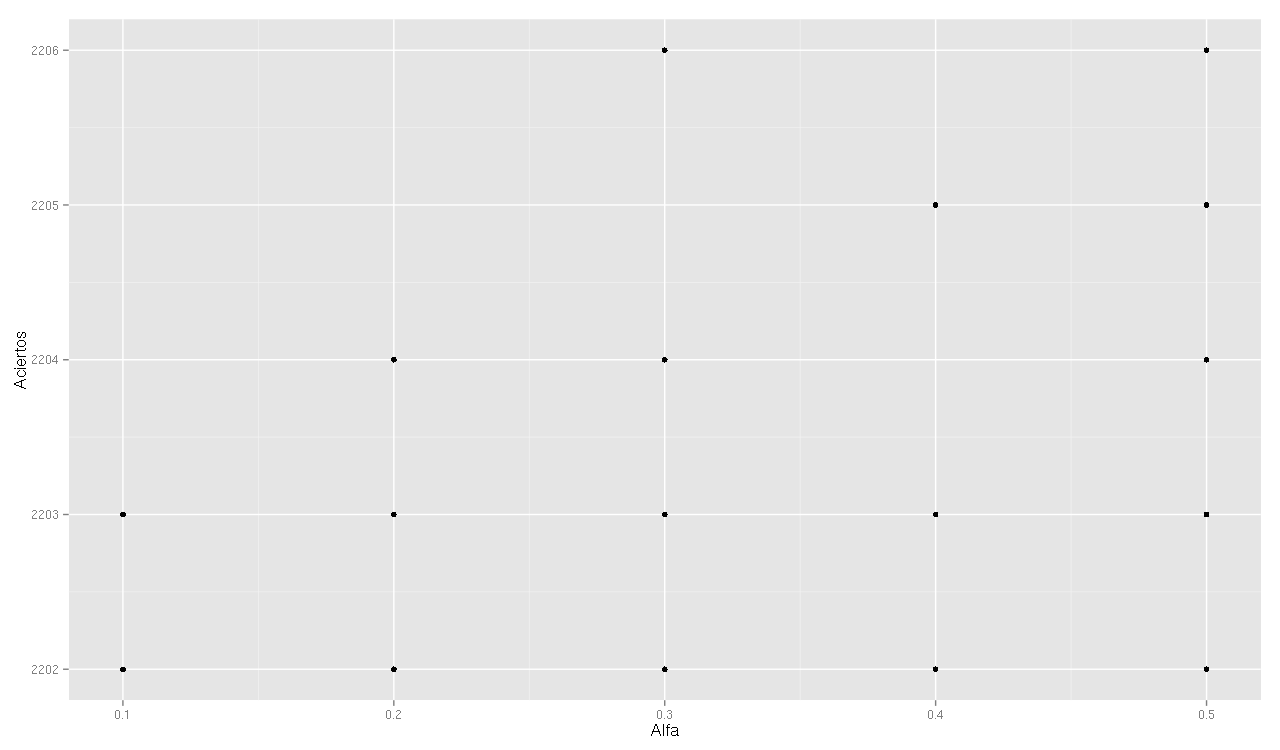
\includegraphics[scale=0.2]{adult_alfa_points_iteracion_iteinal.png}
	  \caption{Comparaci\'on entre el valor del par\'ametro Alfa y el n\'umero de Aciertos}
	  \label{fgr:alfaIteracion}
	\end{figure}

	\begin{figure}[h]
	  \centering
	  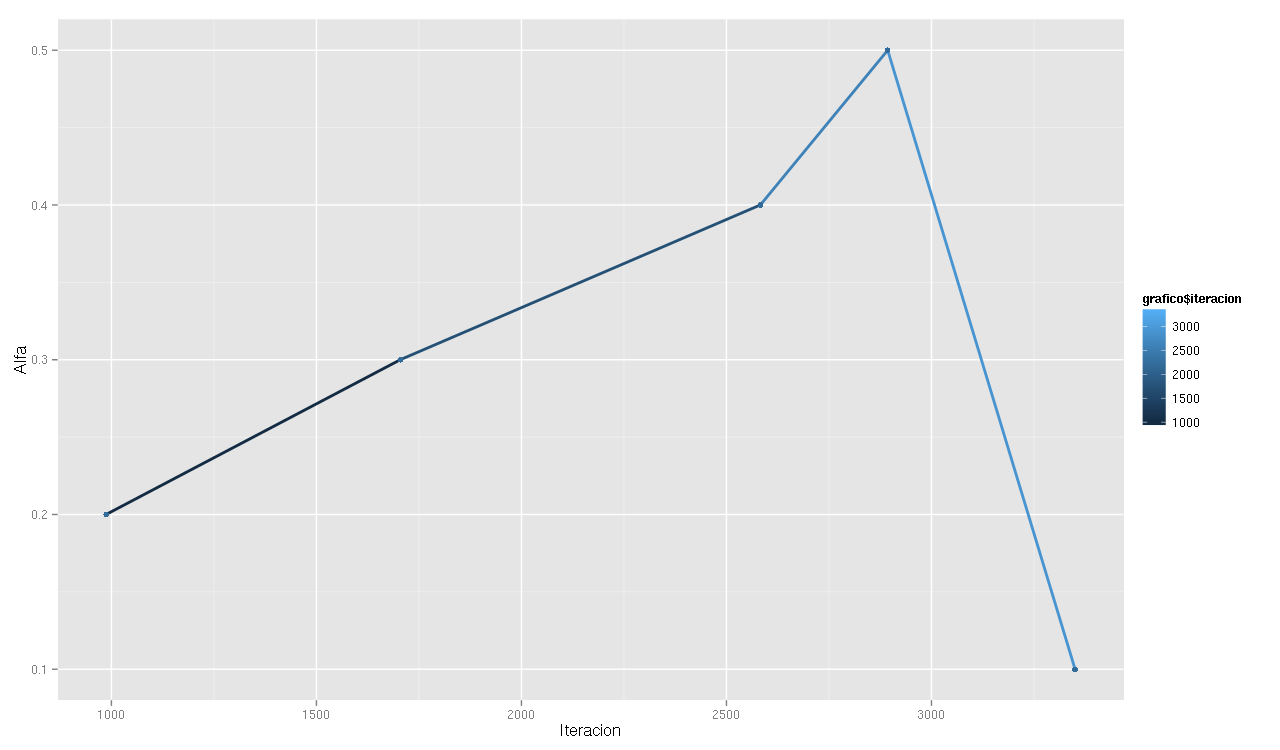
\includegraphics[scale=0.2]{adult_alfa_iteracion_promedio_final.png}
	  \caption{Comparaci\'on entre el valor del par\'ametro Alfa y el n\'umero de Iteraciones}
	  \label{fgr:alfaIteracion}
	\end{figure}

\section{ Resoluci\'on del problema, Escalando los datos linealmente y distintos valores de alfa.}
    De nuevo como en el ejercicio anterior al realizar el escalado de datos se reduce el n\'umero de 
iteraciones, de aproximadamente 2000 a 133 iteraciones como m\'inimo valor, esto puede mejorar el desempeño del perceptr\'on
en casos de tener conjunto de datos con gran n\'umero de patrones. ya que a medida que poseemos m\'as patrones tender\'a
a demorar por el orden de complejidad del algoritmo si bien no es catalogado como un algoritmo NP-hard ya que tiene un orden  de complejidad polinomial,
 el proceso de selecci\'on de pesos se puede hacer m\'as largo a medida que incremente el n\'umero de patrones.
 Un aspecto importante es que a pesar que en algunos valores de alfa no llegaron a discriminar completamente todos los patrones
el n\'umero de aciertos es bastante cercano a los valores de alfa que si discriminaron completamente los patrones.
Y el n\'umero de aciertos va decreciendo mientras m\'as se acerca a valores negativos de alfa.

    \begin{table}[h]
        \small
        \caption{ Alfas, Promedio de Iteraciones, Cantidad de Aciertos (promedios) }
        \label{tbl:example}
        \begin{tabular*}{0.5\textwidth}{@{\extracolsep{\fill}}llll}
        \hline
        Aciertos (Promedio) & alfa & Ite $<$ Max\_It & Ite (Promedio)\\
        \hline
        2202.1 & 0.5 & $10/10$ &  227.8\\
        2202.1  & 0.4 & $10/10$ & 133.2  \\
        2181.8 & 0.3 & $0/10$ &  11000 \\
        2161   & 0.2 & $0/20$ & 11000 \\
        2118  & 0.1 & $0/20$ & 11000 \\
        971  & -0.1 & $0/20$ & 11000 \\
        971  & -0.2 & $0/20$ & 11000 \\
        971  & -0.3 & $0/20$ & 11000 \\
        971  & -0.4 & $0/20$ & 11000 \\
        971  & -0.5 & $0/20$ & 11000 \\
        \hline
        \end{tabular*}
        \end{table}
 Se puede visualizar mejor lo comentado anteriorment  en la figura 5.
	\begin{figure}[h]
	  \centering
	  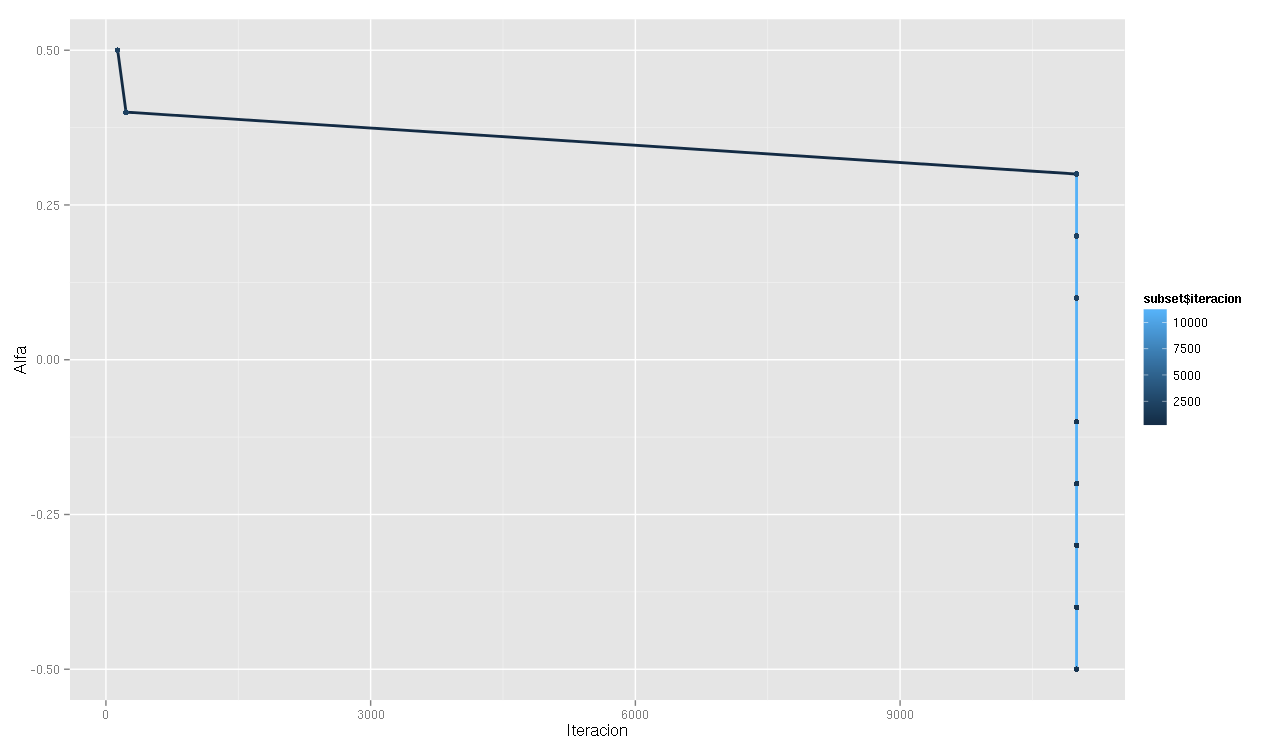
\includegraphics[scale=0.2]{adult_alfa_iteracion_escalado.png}
	  \caption{Comparaci\'on entre el valor del par\'ametro Alfa y el n\'umero de Iteraciones}
	  \label{fgr:alfaIteracion}
	\end{figure}


\section{ Resoluci\'on del problema, Orden de Ingreso de Muestras, muestras de una misma clase, y muestras alternadas y distintos valores de alfa.}

        Cuando los patrones se encuentran alternados por clase se mantienen el n\'umero de iteraciones bajo, a diferencia de 
        colocar todos los patrones que pertenecen a una clase primero, esto lo que genera es incrementar el n\'umero de iteraciones
        haciendo que resuelve de forma m\'as r\'apida y sencilla.

        \begin{table}[h]
        \small
        \caption{ Alfas, Promedio de Iteraciones, Cantidad de Aciertos (promedios) }
        \label{tbl:example}
        \begin{tabular*}{0.5\textwidth}{@{\extracolsep{\fill}}llll}
        \hline
        Aciertos (Promedio) & alfa & Ite $<$ Max\_It & Ite (Promedio)\\
        \hline
        2200 & 0.5 & $20/20$ &  166.4\\
        2200  & 0.4 & $20/20$ & 218.9  \\
        2166 & 0.3 & $0/10$ &  3000 \\
        2148 & 0.2 & $0/10$ &  3000 \\
        2079 & 0.1 & $0/10$ &  3000 \\
        375  & -0.1 & $0/20$ & 3000 \\
        375  & -0.2 & $0/20$ & 3000 \\
        375  & -0.3 & $0/20$ & 3000 \\
        375  & -0.4 & $0/20$ & 3000 \\
        375  & -0.5 & $0/20$ & 3000 \\
        \hline
        \end{tabular*}
        \end{table}

%Footnotes
%\footnotetext{\dag~ Script para formatear Git Hub: [http://bit.ly/15VZJBC].}
%\item \emph{Importar Archivos},


\footnotesize{
%\bibliography{rsc} %your .bib file
%\bibliographystyle{rsc} %the RSC's .bst file
}

\end{document}
